\pagestyle{headings}
\pagenumbering{arabic}
\chapter{Background}
\label{chapter:background}
\section{DNA methylation} 
\label{section:DNAMeth} 
Epigenetics is the name of the science that studies the heritable information not relying on changes in the DNA sequence and influencing the organisms phenotype. There exist two kinds of epigenetic modifications: Chromatin and DNA modifications. Chromatin is the three-dimensional arrangement of DNA and a histone protein. The modification of Chromatin is performed by binding of an amino group or RNA.\cite{Epigenetics}\\

The most common DNA modification is the addition of one methyl group to the fifth position in the cytosine ring of DNA. Methylation occurs mainly at \acp{CpG}, where a cytosine nucleotide (C) is followed by a guanine nucleotide (G) in the DNA sequence.\cite{DNAMethylation} Whereas the majority of CpGs in mammals are methylated, so called \ac{CGI} are rather unmethylated. The \acp{CGI} are associated to gene regulation as they are often located at the promoter region of genes. Hereby, methylation inhibits the gene expression; ensuring that changes in the methylation pattern of the DNA are effecting diseases like cancer.\cite{Handbook} Hypomethylation of repeat elements for example results in an unstable DNA and may increase the risk of cancer; as also the hypermethylation of cancer suppressor genes.\cite{DNAMethylation} Finally, DNA methylation is responsible for genomic imprinting and X-chromosome inactivation, whereby one of the two alleles respectively is transcribed and the other inactivated by methylation. Dysregulation may contribute to diseases like Prader-Willi syndrome, Angelman syndrome and cancer. \cite{Walter}\\

The transfer of the methyl group to the DNA is performed by \acp{DNMT}. Five different \acp{DNMT} are distinguished in mammals: DNMT1, DNMT2, DNMT3A, DNMT3B and DNMT3L.\cite{DNAMethylation}\\
DNMT1 is known as maintanance methyltransferase as its activity is associated with the DNA replication process. Thereby, not only the DNA of the cell is transmitted from one cell generation to another, but also the methylation patterns. DNMT1 has a preference for hemimythelated DNA, which means that one of the opposite \acp{CpG} is methylated and the other unmethylated. Subsequently, DNMT1 transfers the methylation by methylating the positions on the daughter strand that are methylated at the same position on the parental strand.\cite{DNAMethylation}\newline
DNMT2 is negligible if human DNA methylation is considered, because it methylates small RNA at the anticodon loop.\cite{DNMT2}\newline
DNMT3A and DNMT3B are de novo methyltransferases, which work during the early embryonic development to synthesize new methylations. Hereby, the enzymes do not show any preference neither for hemi- or unmethylated DNA nor for a DNA-strand. In other words, DNMT3A/B may add a methyl-group to any non-methylated \ac{CpG} at any DNA-strand. DNMT3L does not catabolize methylation, but increases the binding ability of DNMT3A/B and thus is required for establishing genomic imprinting.\cite{DNAMethylation}\newline
The loss of one of the methyltransferases leads to embryonic lethality.\cite{DNAMethylation}\\

So far a lot is known about the function of \acp{DNMT}, but some properties still remain unexplained:
\begin{itemize}
\item Why and where do the \acp{DNMT} bind?
\item On which conditions does the methylation event depend?
\item Which enzymes are able to methylate multiple \acp{CpG} in a row without deassociating from the DNA?
\item How much de novo and maintenance methylation do DNMT1 and DNMT3A/B perform?
\end{itemize}

To study the function of \acp{DNMT}, a computational, stochastic model is designed and fitted using real biological data.\\

Todo: bisulfite PCR, demethylation, figure CpG

\section{Foundations of statistics} 
\label{section:statistics}
Statistics is a mathematical field, dealing with the development of hypotheses, analysis and organization of empirical data. Here, the data are observations of real experiments, often called the sample data. The denotation sample space $\Omega$ refers to the collection of possible outcomes of the experiment.\cite{Philosophy} Two sections of statistics are distinguishable: descriptive and inferential statistics. Where descriptive statistics summarizes the data without changing it, using statistical methods like mean and standard deviation, inferential statistics is more about analysing data and making predictions based on probability theory.\cite{Introduction}\\
\newtheorem{definition}{Definition}
\begin{definition}[Probability]
The probability P of an event E is the likelihood of an event to happen. P(E) can take any value between zero and one, where zero describes the impossibility and one the certainty of the event to occur.
\end{definition}
\begin{definition}[Conditional Probability]
The conditional probability is the probability of an event to happen, given some prior knowledge K:\newline
$P(E \mid K) := P(E \cap K) / P(K)$ if $P(K) \neq 0$. 
\end{definition}
\begin{definition}[Independence]
Two events A and B are independent if $P(A \mid B) = P(A)$, so if the probability of A does not change compared to the probability of A given B.
\end{definition}
If two events are independent it holds $P(A \cap B) = P(A) + P(B)$ otherwise $P(A \cap B) = P(A) + P(B) - P(A \cup B)$
\begin{definition}[Random Variable (RV)]
A random variable X describes an outcome of an experiment.
\end{definition}
\begin{definition}[Probability Distribution]
The representation of the probability of each value of a \ac{RV} is called a probability distribution.
\end{definition}
Given the Definitions one to five, the data can be described using a stochastic model.
%E(X), V(X)?

\section{Markov models} 
\label{section:MM}
A discrete-time Markov model is a stochastic model that fulfils the Markov property. If the next state can only be determined by the current state and not by the previous one, a chain holds the Markov property. Markov models can be used to describe a process and its development over time.\\

A \textbf{Markov chain} is the simplest Markov model. This chain is a sequence of variables $X_1, X_2, ...$ whose outcomes are random, so called \acp{RV}. Each \ac{RV} has a number of possible outcomes, the state space. Given a set of states $S = \{s_1, ..., s_n\}$ with transitions between the states, $p_{ij}$ is the transition probability from $s_i$ to $s_j$. And P of size $|S|\cdot|S|$ is the transition matrix containing the transition probabilities between all possible combinations of states.\newline
Let $X_0$ be the initial distribution of the chain X s.t. $\sum_{x \in X_0}{x} = 1$, then $X_1 = X_0 * P$ is the distribution of X at time t=1. We call $\pi$ the equilibrium distribution; the distribution of X that does not change from one time step to another or formally: $\pi * P = \pi$.\newline
In general, we distinguish between \acp{CTMC}, which act in continuous time and \acp{DTMC} in discrete time.\\
%characteristics of Markov Chain? Ergodic...
\textbf{\acp{HMM}} are an extension of Markov chains. There are two kinds of states in this model; hidden states S and observable output states O. Similarly, there is a transition probability matrix between the states in S and a matrix of output probabilities B between the hidden and the output states. Figure \ref{HMM} shows a graphic representation of an \ac{HMM}.\newline
This model is used, when there is information about the output of a process, but no knowledge about the states of the system.\\
%Viterbi?
\begin{figure}[h]
\centering
\begin{tikzpicture}[node distance=2cm,>=stealth',bend angle=45,auto,->,shorten >=1pt]
  \tikzstyle{place}=[circle,thick,draw=blue!75,fill=blue!20,minimum size=6mm]
  \tikzstyle{red place}=[place,draw=red!75,fill=red!20]
  	\node [place](S00){S00};
    \node [place](S01)[right of=S00]{S01};
    \node [place](S02)[right of=S01]{S02};
    \node [place](S03)[right of=S02]{S03};
    \node [place](S10)[below of=S00]{S10};
    \node [place](S11)[below of=S01]{S11};
    \node [place](S12)[below of=S02]{S12};
    \node [place](S13)[below of=S03]{S13};
    \node [red place](O0)[below of=S10]{O0};
    \node [red place](O1)[below of=S11]{O1};
	\node [red place](O2)[below of=S12]{O2};
	\node [red place](O3)[below of=S13]{O3};
	\path (S00)edge(S01)
    		   edge(S10)
    		   edge(S11)
    		   edge[bend right](O0)
    	  (S01)edge(S02)
    		   edge(S11)
    		   edge(S12)
    		   edge[bend right](O1)
    	  (S02)edge(S03)
    		   edge(S12)
    		   edge(S13)
    		   edge[bend right](O2)
    	  (S03)edge(S13)
    		   edge[bend right](O3)
    	  (S10)edge(S11)
    		   edge(O0)
    	  (S11)edge(S12)
    		   edge(O1)
    	  (S12)edge(S13)
    		   edge(O2)
    	  (S13)edge(O3);
\end{tikzpicture}
\caption{An HMM with eight hidden states(blue) and four emission states(red).}
\label{HMM}
\end{figure}

\section{Bayesian statistics} 
\label{section:Baystat}
By analysing observed data, one is able to develop a stochastic model which represents the process that generated the observed data. Utilizing Bayesian statistical methods, the parameters of the statistical model can be determined. Thereby, Bayesian statistics make use of the Bayes' theorem.\cite{BayStat}\newline
\begin{definition}[Bayes' Theorem]
Given two events A and B with $P(B) \neq 0$, the conditional probability of the events is given as $P(A \mid B) = (P(B \mid A) * P(A)) / P(B)$.
\end{definition}
Here, P(A) is the prior probability of A, so our expectation about the process without the knowledge of additional information. $P(A \mid B)$ is called the posterior probability, the probability of A, taking B into account. Finally, $P(B \mid A)$ is the likelihood function; the probability of B, given that A is true.\newline
The likelihood is an important function in Bayesian statistics. By maximizing the likelihood function, the most probable parameter of a model given an observation are observed. Because of the importance of the likelihood function, it is also defined as 
\begin{equation}
L(\Theta \mid x_0,...,x_n) = P_{\Theta}(x_0) * ... * P_{\Theta}(x_1).
\end{equation}
The process of determining the parameter $\Theta$ that maximizes the likelihood function given the data ${x_0,...,x_n}$ is called \textbf{\ac{MLE}}.\\

In the following, we describe the two major techniques in Bayesian statistics; \ac{MCMC} and \ac{ABC}.\\

The term \textbf{\ac{MCMC}} describes a collection of algorithms which simulate the distribution of a Markov chain after some time t. Once, the initial distribution $X_0$ and the transition matrix P are known, the simulation works by sampling from these distributions. Therefore, a random number is generated and based on the number, the state of the chain is identified, depending on in which range of the distribution the value is falling.\newline
E.g. assuming, we have three dice, two dice are biased and one regular. We want to compute the probability of throwing six pips. We choose randomly between the biased and the regular dice. The probability distribution of dice selecting is defined by $X_0$; the probability to dice six pips can be retrieved by considering the transition matrix P.
%\begin{figure}[h]
\begin{center}
%\centering
\begin{large}
$X_0$ =
\end{large}
$\begin{blockarray}{cccc}
  & dice 1 & dice 2 & dice 3 \\
  \begin{block}{c[ccc]}
    & 1/3 & 1/3 & 1/3 \\
  \end{block}
\end{blockarray}$
%\caption{initial distribution $X_0$}
%\end{figure}
%\begin{figure}[h]
%\centering
\\
\begin{LARGE}
P =
\end{LARGE}
$\begin{blockarray}{ccccccc}
  & 1 & 2 & 3 & 4 & 5 & 6 \\
  \begin{block}{c[cccccc]}
    dice 1 & 2/15 & 2/15 & 2/15 & 2/15 & 2/15 & 1/3 \\
    dice 2 & 1/3 & 1/12 & 1/12 & 1/12 & 1/6 & 1/4 \\
    dice 3 & 1/6 & 1/6 & 1/6 & 1/6 & 1/6 & 1/6 \\
  \end{block}
\end{blockarray}$
%\caption{transition matrix P}
%\end{figure}
\end{center}
The simulation starts by generating the first random number between zero and one. If the value falls into the first interval of $X_0$, we choose the first dice. Otherwise, if the value is greater than 1/3, but smaller than 2/3, so if the value falls in the second interval, we choose the second dice. If that also does not hold, we select dice three.\newline
After initializing the dice, the rolling of the dice is simulated by generating random variates again. The row, which represents the selected dice, gives the probability distribution of pips. If we roll dice one or two, the probability of throwing six pips is higher than if we rolled dice three. By repeating the simulation multiple times, we get a specific distribution of pips for each combination of selected dice. Comparing a real experiment with multiple throws to our simulated distribution, we are able to predict the dice used in the experiment. Figure \ref{MCMC} shows the pseudo-code of one simulation run of an MCMC.
\begin{figure}
\begin{algorithmic}
\State $r \gets random(0,1)$
\For {$i \in len(X_0)$}
\If {$r \leq X_0[i]$}
\State $dice \gets i$
\State break
\Else
\State $r \gets r - X_0[i]$
\EndIf
\EndFor
\State $r \gets random(0,1)$
\For {$i \in len(P[dice])$}
\If {$r \leq P[dice][i]$}
\State $pips \gets i$
\State break
\Else
\State $r \gets r - P[dice][i]$
\EndIf
\EndFor
\end{algorithmic}
\label{MCMC}
\end{figure}

A second method in computer simulations is \textbf{\ac{ABC}}. In contrast to \ac{MCMC}, \ac{ABC} does not need to evaluate the likelihood function, which may be an advantage because the evaluation is computational costly and sometimes not possible. Instead, the similarity of the observed to the real data is measured with a distance function. Hereby, samples are drawn from the prior distribution. If the distance of the sample to the desired value is greater than a threshold, the sample is rejected, otherwise it is accepted. The posterior distribution results from the set of accepted samples (see figure \ref{ABC} for the pseudo-code).\cite{ABC}
\begin{figure}[h]
\begin{algorithmic}
\State $sim \gets prior()$
\If {$dist(sim,data) < \epsilon$}
\State accept sim
\Else
\State reject sim
\EndIf
\end{algorithmic}
\label{ABC}
\end{figure}

\section{Problem} 
\label{section:Problem}
In the context of \acp{DNMT}, Markov models are used to simulate the function of these enzymes, making use of results from biological experiments. Here, few is known about the properties of methyltransferases. Under which condition does the enzyme bind to the DNA and when does it methylate? But the methylation patterns before and after the catabolism of the \acp{DNMT} are known. From the methylation pattern distribution, a sequence of methylation states can be retrieved. Each methylation (unmethylated, hemimethylated, methylated) of one \ac{CpG}-dyad is an output state, whereas the binding state and methylation conditions of the \ac{DNMT} at each \ac{CpG} are hidden states. Thus the traversing probabilities between the hidden states P are equal to the probabilities of the \acp{DNMT} to bind/fall of and the output probabilities represent the different methylation probabilities.\\
Given the output sequence\newline
\begin{align}
O_i := \text{methylation state of CpG-dyad i}\\
O_i = \left\{
\begin{array}{l}
\text{unmethylated} \\
\text{hemimethylated} \\
\text{methylated,}
\end{array}
\right.\newline
\end{align}
we are able to determine the most likely sequence of S\newline
$S_i := \text{state of DNMT at CpG i}$\newline
%Moreover, P and B can be reconstructed by computer simulation of the \ac{DTMC}.
Moreover, our goal is to determine\newline
\begin{align}
P := \text{probability of DNMT to change binding state}\\
B := \text{methylation probabilities.}
\end{align}
Figure \ref{fig:methylationpatterns} shows the four kind of methylation patterns.\\
\begin{figure}[h]
\begin{subfigure}{.5\textwidth}
\centering
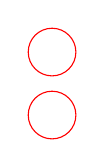
\begin{tikzpicture}
  \draw[red](0,0)circle(2ex);
  \draw[red](0,-0.8)circle(2ex);
\end{tikzpicture}
\caption{}
\label{fig:sfig0}
\end{subfigure}%
\begin{subfigure}{.5\textwidth}
\centering
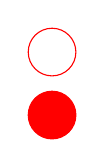
\begin{tikzpicture}
  \draw[red](0,0)circle(2ex);
  \draw[red, fill=red](0,-0.8)circle(2ex);
  \end{tikzpicture}
  \caption{}
  \label{fig:sfig1}
\end{subfigure}
\begin{subfigure}{.5\textwidth}
\centering
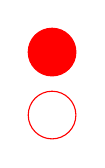
\begin{tikzpicture}
  \draw[red, fill=red](0,-0.2)circle(2ex);
  \draw[red](0,-1)circle(2ex);
  \end{tikzpicture}
  \caption{}
  \label{fig:sfig2}
\end{subfigure}
\begin{subfigure}{.5\textwidth}
\centering
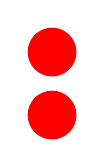
\begin{tikzpicture}
  \draw[red,fill=red](0,-0.2)circle(2ex);
  \draw[red,fill=red](0,-1)circle(2ex);
  \end{tikzpicture}
  \caption{}
  \label{fig:sfig3}
\end{subfigure}
\caption{Kind of methylation patterns; each figure shows a CpG/CpG-dyad on the parental and the daughter strand; each circle represents one CpG; plane red circles are methylated CpGs; (a) unmehtylated, (b) hemimethylated (upper strand unmethylated, lower strand methylated), (c) hemimethylated (vice versa), (d) fully methylated CpGs}
\label{fig:methylationpatterns}
\end{figure}

Recently, different models and computational approaches were studied in order to predict the methylation process. Here we present some of them.\\

\section{Related work} 
\label{section:RelWork}
One example of such a model to study the methylation activity of \ac{DNMT} was introduced by Genereaux et al. in 2005. Using bisulfite \ac{PCR} newly synthesized methylations on both strands were discovered, which cannot both result from the malfunction of maintenance methylation. Maintenance methylation occurs only on the daughter strand and independent on which strand is the daughter strand, the origin of the mathylation of the other strand is unclear. Thus, the authors assume that de novo methylation exists and develop a model, where $\mu$ represents the maintenance methylation rate and $\delta_p$ and $\delta_d$ the de nove methylation rate at the parent and daughter strand respectively. The methylation state of each \ac{CpG}-dyad is either M, H or U (methylated, hemimethylated, unmethylated), whereas the state of a single \ac{CpG} is either m (methylated) or u (unmethylated). Given the methylation rates, the methylation state at time t can be rewritten depending on the previous state like in equations \ref{UHM}.\cite{Genereaux}
\begin{align}
M_t = \mu * m_{t-1} + \delta_d * \delta_p * u_{t-1}\\
H_t = \delta_d * (1- \delta_p) * u_{t-1} + \delta_p * (1- \delta_d) * u_{t-1} + (1-\mu) * m_{t-1}\\
U_t = (1- \delta_p) * (1- \delta_d) * u_{t-1},
\label{UHM}
\end{align}
where (1-x) is the rate of a specific methylation not happening.\newline
By rewriting the equations above, an equations for the equilibrium distribution of the methylation states can be retrieved. Additionally, the likelihood of the states can be computed given the methylation rates.\cite{Genereaux}\\

Fu et al. used the same model and data from double-stranded DNA to infer the methylation parameters, considering errors in the methylation measuring process. These errors may occur during bisulfite conversion. Regularly, unmethylated cytosines are converted to uracil and methylated cytosines recognized. In the opposite case, unmethylated cytosines are not converted or methylated cytosines falsely converted. The experiments supports the assumption that de novo methylation occurs on both strands. Moreover, the authors come to the conclusion that the methylation rates do not follow their prior distribution, but seems to be location dependant.\cite[errors]\\

Another approach which includes bisulfite conversion errors in its model was introduced by Arand et al..\cite{Wolf} They developed a \ac{HMM} similar to \ac{DTMC} proposed by Sontag, Lorincz and Luebeck.\cite{Sontag} The transition matrix of the Markov Chain is composed of three transition matrix'; one represents the de novo probability, one the maintenance probability and one the strand segregation probabilities. Based on this model, the equilibrium distribution and the methylation level depending on the methylation probability can be computed. Contrary to Sontag, Lorincz and Lubeck, Arand et al. did not compute the maximal methylation probabilities, but the methylation rates and the influence of bisulfite conversion errors using a maximum likelihood approach.\cite{Wolf}\\

Recently, Giehr et al. developed a similar \ac{HMM}, which also includes the hydroxylation probability.TODO... An idea, which we will not enlarge upon in the following.\cite{Giehr}\\